\section{Auswertung}
\subsection{Quadratischer Stab bei einseitiger Aufhängung}

Vor der Bestimmung des Elastizitätsmoduls muss zunächst das Material des Stabes bestimmt werden.
Das geschieht über die Dichte des Stabes, welche mit folgender Formel bestimmt werden kann:

\begin{equation}
  \rho = \frac{m}{V} = \frac{m}{L \cdot b^2}
\end{equation}

Die geometrischen Abmessungen des quadratischen Stabes sind:

\begin{enumerate}
  \item Länge: L=\SI{55}{\centi\meter} = \SI{0.55}{\meter}
  \item Masse: m=\SI{435.5e-3}{\kilo\gram}
  \item Breite:
    \begin{enumerate}
      \item Messwerte: \SI{10.4}{\milli\meter}, \SI{10.1}{\milli\meter},
      \SI{10.2}{\milli\meter}, \SI{10.1}{\milli\meter}, \SI{10.1}{\milli\meter},
      \SI{10.1}{\milli\meter}, \SI{10.1}{\milli\meter},
      \SI{10.1}{\milli\meter}, \SI{10.1}{\milli\meter}, \SI{10.1}{\milli\meter}
      \item Mittelwert: b = \SI{10.14(3)e-3}{\meter}
    \end{enumerate}
\end{enumerate}

Der Mittelwert der Breite wird mit dieser Gleichung bestimmt:

\begin{equation}
  \bar{x} = \frac{1}{N} \sum_{i=0}^{N} x_i
\end{equation}

Daraufhin wird die Standartabweichung von dem Mittelwert ermittelt:

\begin{equation}
  \sigma = \frac{1}{\sqrt{N}\sqrt{N-1}} \sqrt{\sum_{i}(x_i-\bar{x})^2}
\end{equation}

Nun ergibt sich für den quadratischen Stab die Dichte:\\
\centerline{$\rho = 7701,04 \pm 45,57 \si[per-mode=fraction]{\kilo\gram\per\metre\tothe{3}}$}

Der Fehler der Dichte lässt sich mithilfe der Gauß´schen Fehlerfortpflanzung berechnen:

\begin{equation}
  \Delta \rho = \sqrt{\left(\frac{\partial\rho}{\partial b} \cdot \Delta b \right)^2}
\end{equation}

Wenn dieser Wert mit Literaturwerten verglichen wird folgt, dass die Dichte von Eisenstahl
am ähnlichsten ist.\\
\centerline{$\rho_{ES} = 7700 \si[per-mode=fraction]{\kilo\gram\per\metre\tothe{3}}$}


Mithilfe der Messwerte, die in Tabelle 1 dargestellt sind, lässt sich nun eine
Ausgleichsrechnung durchführen um das Elastizitätsmodul zu bestimmen. Dafür wird die
Durchbiegung D(x) und $\left( Lx^2- \frac{x^3}{3} \right)$ im Plot aufgetragen.
Die Ausgleichsgerade wird mithilfe von Python 3.6 bestimmt.
Die Parameter der Ausgleichsgerade sind:\\

\begin{equation}
  y=mx+b
\end{equation}

\begin{itemize}
  \item m = \SI{33.557(547)e-3}{\meter\tothe{-2}}
  \item b = \SI{5.45(224)e-5}{\meter}
\end{itemize}

Durch Vergleichen von den Gleichungen (5) und (18) folgt für das Elastizitätsmodul:\\

\begin{equation}
  m = \frac{F}{2EI} \iff E= \frac{F}{2mI}
\end{equation}

Das Flächenträgheitsmoment $I$ lässt sich mit der oben genannten Formel bestimmen:\\

\centerline{$I_{quadrat} = \frac{b^4}{12} = \SI{8.81(10)e-10}{\meter\tothe{4}}$}

Der Fehler wird wieder mit der Gauß´schen Fehlerfortpflanzung bestimmt, wie bei Gleichung (17).\\

\begin{table}
  \centering
  \caption{Tabelle mit Messdaten und Daten für die Ausgleichsrechnung}
  \begin{tabular}{c c c}
    \toprule
    x in \si{\meter} & D(x) in $10^{-3}\si{\meter}$ & $\left(Lx^2-\frac{x^3}{3}\right) \text{in} \, 10^{-3}\si{\meter}$ \\
    \midrule
    0.03 & 0.03 &  0.486 \\
    0.05 & 0.04 &  1.33 \\
    0.10 & 0.24 &  5.17 \\
    0.15 & 0.47 &  11.25 \\
    0.20 & 0.75 &  19.33 \\
    0.25 & 1.07 &  29.17 \\
    0.30 & 1.4 &  40.5 \\
    0.35 & 1.88 &  53.08 \\
    0.40 & 2.22 &  66.66 \\
    0.45 & 2.78 &  81 \\
    \bottomrule
  \end{tabular}
\end{table}

\begin{figure}[H]
  \centering
  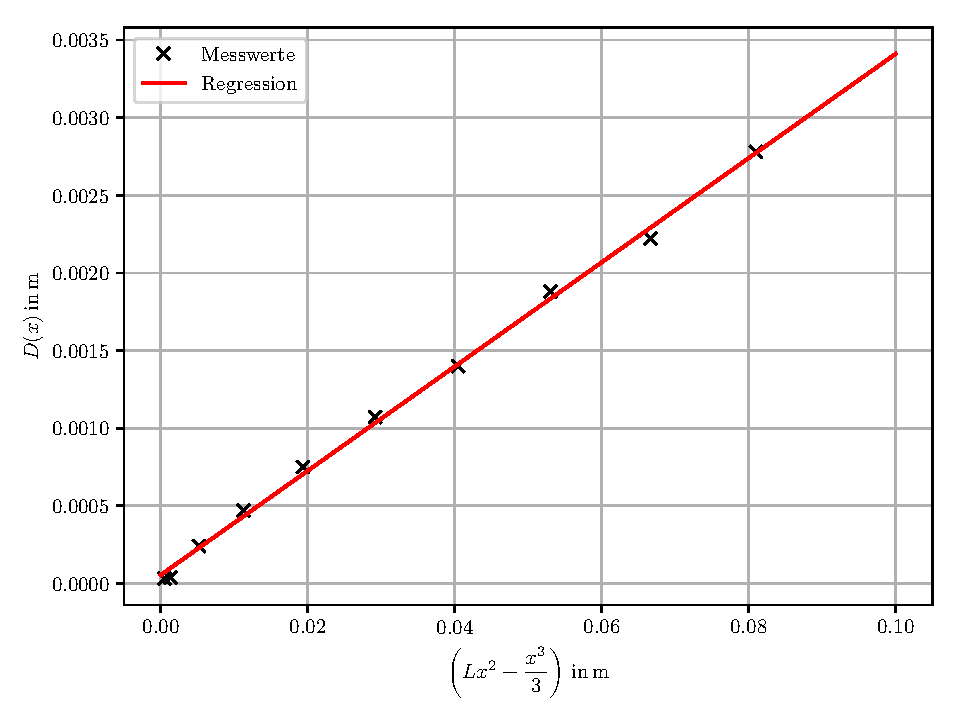
\includegraphics[width=\textwidth]{ausgleichsgerade1.pdf}
  \caption{Messwerte des quadratischen Stabes mit linearer Regression}
\end{figure}

Die Kraft F ist die Gewichtskraft des verwendeten Gewichtes. In diesen Fall ist das Gewicht
$m_0 = \SI{534.5e-3}{\kilo\gram}$ also ergibt sich für die Gewichtskraft:\\
\centerline{$F = m_0 \cdot g = 5,234 N$}

Nun lässt sich das Elastizitätsmodul des quadratischen Stabes bestimmen und der Fehler
wird wieder mit der Gauß´schen Fehlerfortpflanzung berechnet:

\begin{equation}
  \Delta E = \sqrt{\left(\frac{\partial E}{\partial m} \cdot \Delta m \right)^2 +
  \left( \frac{\partial E}{\partial} I \cdot \Delta I \right)^2}
\end{equation}

Also ist das Elastizitätsmodul: \\
\centerline{$E = \num{88.7(18)e9} \frac{N}{m^2}$}

\subsection{Runder Stab mit einseitiger Aufhängung}

Bei dem Runden Stab muss zunächst wieder die Dichte bestimmt werden um das Material
ungefähr bestimmen zu können. Die geometrischen Abmessungen des runden Stabes sind:

\begin{enumerate}
  \item Länge L = \SI{0.55}{\meter}
  \item Masse m = \SI{121.3e-3}{\kilo\gram}
  \item Durchmesser:
  \begin{enumerate}
    \item Messwerte: \SI{10}{\milli\meter}, \SI{10}{\milli\meter}, \SI{10}{\milli\meter},
    \SI{10}{\milli\meter}, \SI{10}{\milli\meter}, \SI{10}{\milli\meter},
    \SI{10}{\milli\meter}, \SI{10}{\milli\meter}, \SI{10}{\milli\meter},
    \SI{10}{\milli\meter}, \SI{10}{\milli\meter}
    \item Mittelwert: d = \SI{10e-3}{\meter}
  \end{enumerate}
\end{enumerate}

Der Mittelwert wird mithilfe der Gleichung (15) berechnet aber da alle Messwerte gleich
sind ist der Mittelwert das gleiche wie die Messwerte und hat keinen Fehler.

Die Dichte des runden Stabes lässt sich nun mit der folgenden Gleichung bestimmen:

\begin{equation}
  \rho = \frac{m}{V} = \frac{m}{L \pi \frac{d^2}{4}}
\end{equation}

Somit ergibt sich für die Dichte:\\
\centerline{$\rho = \SI[per-mode=fraction]{2808.07}{\kilo\gram\per\meter
\tothe{3}}$}

Diese Dichte wird wieder mit Literaturwerten verglichen und es folgt, dass die Dichte
von Aluminium am ähnlichsten ist:\\
\centerline{$\rho_A = \SI[per-mode=fraction]{2710}{\kilo\gram\per\meter
\tothe{3}}$}

\begin{table}
  \centering
  \caption{Tabelle mit Messdaten und Daten für die Ausgleichsrechnung}
  \begin{tabular}{c c c}
  \toprule
  $x$ in \si{\meter} & $D(x) \text{in} \, 10^{-3}\si{\meter}$ & $\left(Lx^2-\frac{x^3}{3}\right) \text{in} \, 10^{-3}\si{\meter}$ \\
  \midrule
  0.03 & 0.05 &   0.486 \\
  0.05 & 0.1 & 1.33 \\
  0.10 & 0.42 &   5.17 \\
  0.15 & 0.82 &   11.25 \\
  0.20 & 2.1  & 19.33 \\
  0.25 & 1.99 &   29.17 \\
  0.30 & 2.62 &   40.5 \\
  0.35 & 3.42 &   53.08 \\
  0.40 & 4.13 &   66.66 \\
  0.45 & 4.93 &   81 \\
  \bottomrule
  \end{tabular}
\end{table}

In der Tabelle 2 sind die Messwerte für den runden Stab dargestellt. Nun wird wieder
die Durchbiegung D(x) und die Werte zum Term $\left(Lx^2-\frac{x^3}{3}\right)$ in
einem Plot dargestellt und es wird eine Ausgleichsrechnung durchgeführt.

\begin{figure}[H]
  \centering
  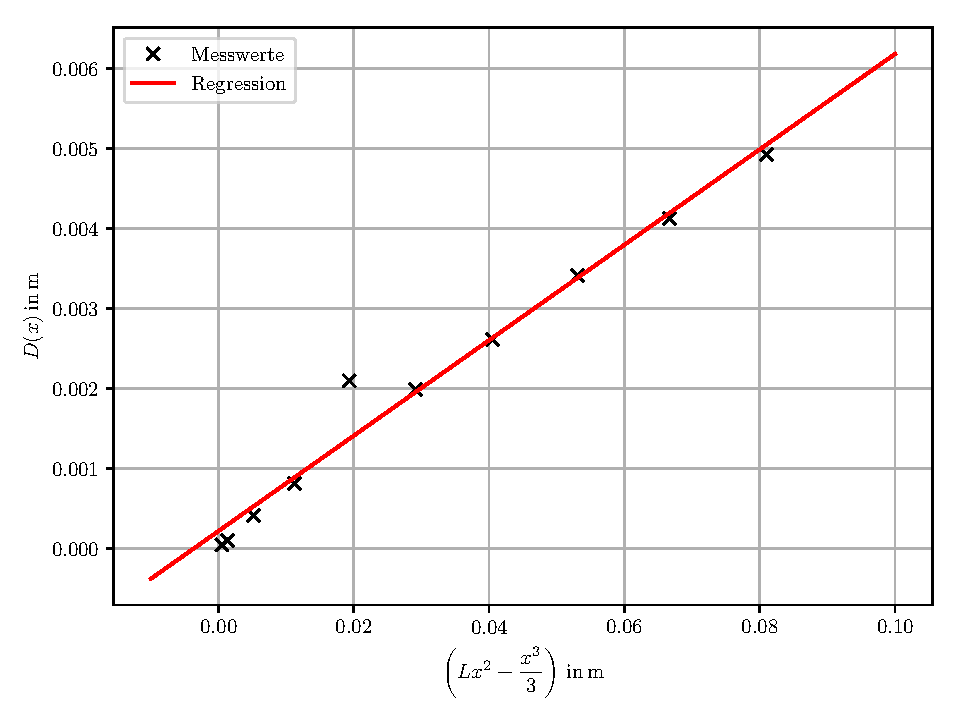
\includegraphics[width=\textwidth]{ausgleichsgerade2.pdf}
  \caption{Messwerte des runden Stabes mit linearer Regression}
\end{figure}

Die Parameter der Ausgleichsgeraden werden wieder mithilfe von Python 3.6 ermittelt:

\begin{itemize}
  \item m = \SI{59.623(3313)e-3}{\meter\tothe{-2}}
  \item b = \SI{22.17(1559)e-5}{\meter}
\end{itemize}

Durch Vergleichen der Gleichungen (5) und (18) ergibt sich wieder die Gleichung (19).

Die Formel für das Flächenträgheitsmoment eines runden Stabes lässt sich auch mit
der oben genannten Gleichung ermitteln:\\

\centerline{$I_{Rund} = \frac{\pi}{4} \frac{d}{2}^4 = \SI{490.87e-12}{\meter\tothe{4}}$}

Die Gewichtskraft für den runden Stab ist die gleiche wie bei dem quadratischen,
da die Masse des Gewichtes gleich ist. F ist also $5,243N$.

Das Elastizitätsmodul des runden Stabes lässt sich nun bestimmen und der Fehler
wird mit der Gleichung (19) berechnet.\\

\centerline{$E = \num{90(5)e9} \frac{N}{m^2}$}

\subsection{Quadratischer Stab mit beidseitiger Aufhängung}

Bei der Bestimmung des Elastizitätsmoduls durch beidseitige Aufhängung müssen zwei
Fälle betrachtet werden. Zunächst wird die Durchbiegung von $0$ bis $\frac{L}{2}$
durch die Gleichung (12) beschrieben. Der Teil von $\frac{L}{2}$ bis $L$ wird seperat
durch die Gleichung (13) beschrieben.

Für beide Hälften des Stabes lässt sich nun eine Ausgleichsrechnung durchführen
und jeweils ein Elastizitätsmodul bestimmen. Im idealfall sollten die
Elastizitätsmodule gleich sein.

Zunächst wird das Elastizitätsmodul für $0$ bis $\frac{L}{2}$ bestimmt.

\begin{table}
  \centering
  \caption{Tabelle mit Messdaten und Daten von $0$ bis $\frac{L}{2}$}
  \begin{tabular}{c c c}
    \toprule
    x in \si{\meter} & $D(x) \text{in} \, 10^{-3} \si{\meter}$ &
    $ \left( 3L^2x-4x^3 \right) \text{in} \, 10^{-3} \si{\meter}$\\
    \midrule
    0    & -0.03 & 0 \\
    0.05 & 0.24 & 44.87 \\
    0.10 & 0.42 & 86.75 \\
    0.15 & 0.66 & 122.625 \\
    0.20 & 0.89 & 149.5 \\
    0.25 & 0.88 & 164.375 \\
    \bottomrule
  \end{tabular}
\end{table}

\begin{figure}[H]
  \centering
  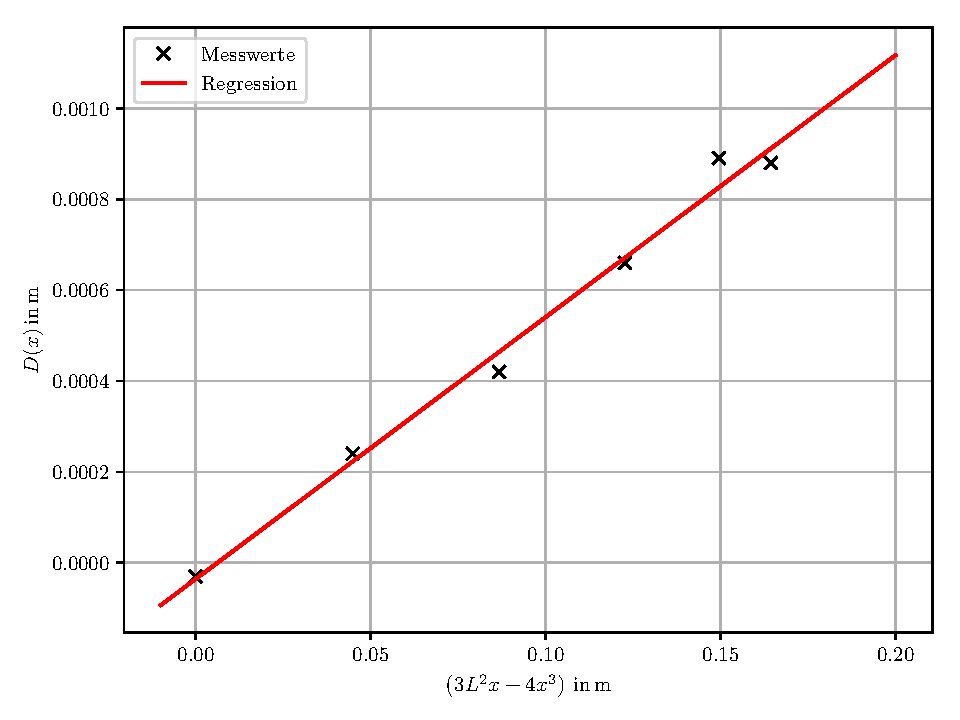
\includegraphics[width=\textwidth]{ausgleichsgerade3.pdf}
  \caption{Messwerte des quadratischen Stabes für $0$ bis $\frac{L}{2}$ mit linearer Regression}
\end{figure}

Die Ergebnisse der Ausgleichsrechnung, die wieder mit Python 3.6 durchgeführt wurde,
lauten:

\begin{itemize}
  \item $m = \SI{5.761(305)e-3}{\meter\tothe{-2}}$
  \item $b = \SI{-3.6(34)e-5}{\meter}$
\end{itemize}

Für die Berechnung des Elastizitätsmoduls werden die Gleichungen (18) und (12)
verglichen. Dadurch ergibt sich wieder die Gleichung (19) für das Elastizitätsmodul.
Das Flächenträgheitsmoment für den quadratischen Stab wurde bereits berechnet.

Die Gewichtskraft ist diesmal jedoch anders, da die Masse $m_1 = \SI{2.362}{\kilo\gram}$
beträgt. Daraus ergibt sich dann die Kraft $F = 23,171N$.

Nun lässt sich das Elastizitätsmodul für den ersten Teil der Messung bestimmen,
wobei der Fehler wieder mit der Gleichung (19) berechnet wird:

\centerline{$E = \num{90(5)e9} \frac{N}{m^2}$}

Für den zweiten Teil der Messung von $\frac{L}{2}$ bis $L$ sind die Rechnungen
identisch nur, dass die Gleichung (13) anstatt (12) verwendet wird.

\begin{table}
  \centering
  \caption{Tabelle mit Messdaten und Daten von $\frac{L}{2}$ bis $L$}
  \begin{tabular}{c c c}
    \toprule
    x in \si{\meter} & $D(x) \text{in} \, 10^{-3} \si{\meter}$ &
    $ \left( 4x^3-12Lx^2+9L^2x-L^3 \right) \text{in} \, 10^{-3} \si{\meter}$\\
    \midrule
    0.30 & 1.73 & 164.375 \\
    0.35 & 1.67 & 149.5 \\
    0.40 & 1.57 & 122.625 \\
    0.45 & 1.37 & 86.75 \\
    0.50 & 1.15 & 44.875 \\
    \bottomrule
  \end{tabular}
\end{table}

\begin{figure}[H]
  \centering
  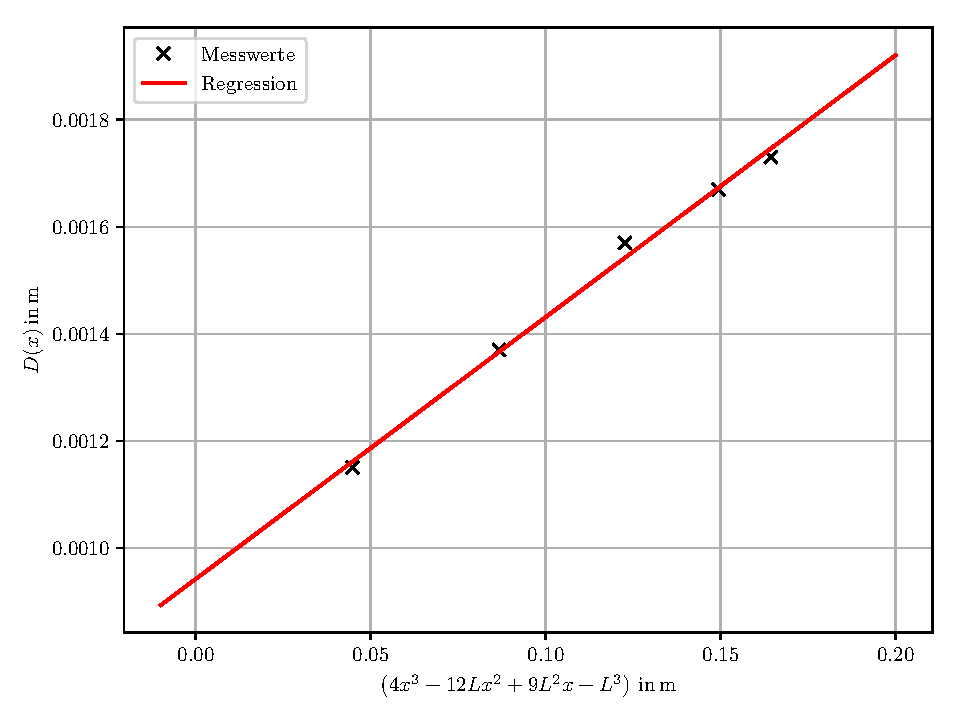
\includegraphics[width=\textwidth]{ausgleichsgerade3.1.pdf}
  \caption{Messwerte des quadratischen Stabes für $\frac{L}{2}$ bis $L$ mit linearer Regression}
\end{figure}

Damit lauten die Parameter der Ausgleichsgeraden, die mit Python 3.6 bestimmt wurden:

\begin{itemize}
  \item $m = \SI{4.893(207)e-3}{\meter\tothe{-2}}$
  \item $b = \SI{94.2(25)e-5}{\meter}$
\end{itemize}


Da alle Rechnungen gleich sind lässt sich sofort das Elastizitätsmodul für den
zweiten Teil der Messungen angeben:\\

\centerline{$E = \num{112(5)e9} \frac{N}{m^2}$}


\subsection{Runder Stab mit beidseitiger Aufhängung}

Für die Bestimmung des Elastizitätsmoduls für den runden Stab bei beidseitiger
Aufhängung müssen wieder zwei Ausgleichsrechnungen durchgeführt werden, für
$0$ bis $\frac{L}{2}$ und für $\frac{L}{2}$ bis $L$. Die verwendeten Formeln sind
die gleichen wie bei dem quadratischen Stab.

Zunächst wird für den ersten Fall $0$ bis $\frac{L}{2}$ die Ausgleichsrechnung
durchgeführt.

\begin{table}
  \centering
  \caption{Tabelle mit Messdaten und Daten von $0$ bis $\frac{L}{2}$}
  \begin{tabular}{c c c}
    \toprule
    x in \si{\meter} & $D(x) \text{in} \, 10^{-3} \si{\meter}$ &
    $ \left( 3L^2x-4x^3 \right) \text{in} \, 10^{-3} \si{\meter}$\\
    \midrule
    0    & 0    &  0 \\
    0.05 & 0.6 & 44.87 \\
    0.10 & 1.02 &  86.75 \\
    0.15 & 1.47 &  122.625 \\
    0.20 & 1.76 &  149.5 \\
    0.25 & 1.92 &  164.375 \\
    \bottomrule
  \end{tabular}
\end{table}

\begin{figure}[H]
  \centering
  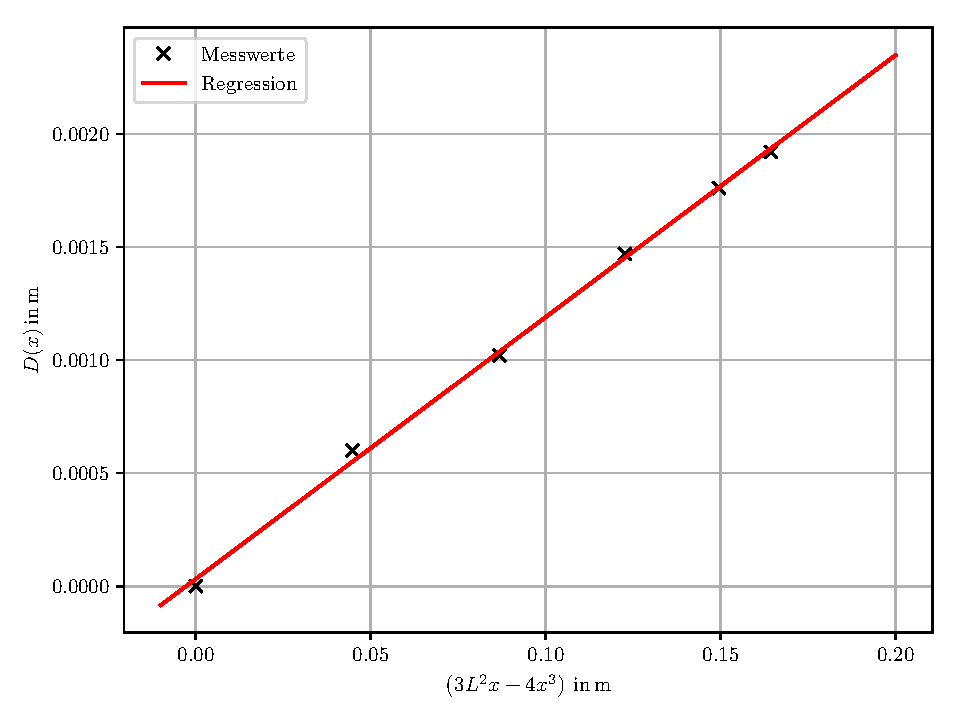
\includegraphics[width=\textwidth]{ausgleichsgerade4.pdf}
  \caption{Messwerte des runden Stabes für $0$ bis $\frac{L}{2}$ mit linearer Regression}
\end{figure}

Nun wird die Ausgleichsrechnung mithilfe von Python 3.6 durchgeführt, womit die Parameter
der Ausgleichsgeraden bestimmt wird:

\begin{itemize}
  \item $m = \SI{11.580(229)e-3}{\meter\tothe{-2}}$
  \item $b = \SI{3.2(25)e-5}{\meter}$
\end{itemize}

Die Rechnungen und Formeln zur bestimmung des Elastizitätsmoduls sind identisch mit
denen die für den quadratischen Stab benutzt wurden. Deshalb lässt sich das Elastizitätsmodul
direkt angeben:

\centerline{$E= \num{84.9(22)e9} \frac{N}{m^2}$}

Das Vorgehen für die Bestimmung des Elastizitätsmoduls für den zweiten Teil der
Messungen ist wieder gleich mit dem für den quadratischen Stab.

\begin{table}
  \centering
  \caption{Tabelle mit Messdaten und Daten von $\frac{L}{2}$ bis $L$}
  \begin{tabular}{c c c}
    \toprule
    x in \si{\meter} & $D(x) \text{in} \, 10^{-3} \si{\meter}$ &
    $ \left( 4x^3-12Lx^2+9L^2x-L^3 \right) \text{in} \, 10^{-3} \si{\meter}$\\
    \midrule
    0.30 & 2.77 &  164.375 \\
    0.35 & 2.64 &  149.5 \\
    0.40 & 2.36 &  122.625 \\
    0.45 & 1.91 &  86.75 \\
    0.50 & 1.4 & 44.875 \\
    \bottomrule
  \end{tabular}
\end{table}

\begin{figure}[H]
  \centering
  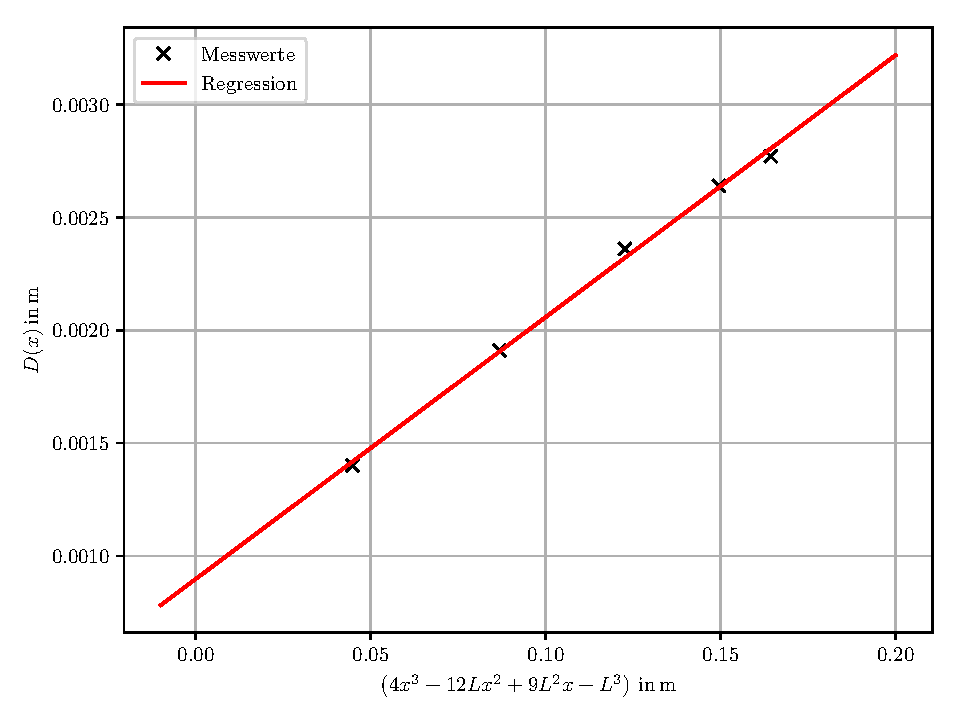
\includegraphics[width=\textwidth]{ausgleichsgerade4.1.pdf}
  \caption{Messwerte des runden Stabes für $\frac{L}{2}$ bis $L$ mit linearer Regression}
\end{figure}

Mithilfe der Messwerte, die in Tabelle 1 dargestellt sind, lässt sich nun eine
Ausgleichsrechnung durchführen um das Elastizitätsmodul zu bestimmen. Die Ausgleichsgerade
wird mithilfe von Python 3.6 bestimmt.

\begin{itemize}
  \item $m = \SI{11.599(337)e-3}{\meter\tothe{-2}}$
  \item $b = \SI{89.8(41)e-5}{\meter}$
\end{itemize}


Damit lässt sich nun das Elastizitätsmodul des runden Stabes noch einmal bestimmen,
mithilfe der Überlegungen für den quadratischen Stab:

\centerline{$E= \num{84.8(25)e9} \frac{N}{m^2}$}
